\chapter{}

\section{The Notion of Being Far}
In the previous chapter we were given an introduction the field of property testing in which the typical kind of problems we are trying to solve are a relaxed form of \textbf{decision problems}.
In decision problems in their non-relaxed form, we given a language \(L\) and an instance (formally: a word) \(x\) and ask whether \(x \in L\).
In the relaxed form of the decision problem as used in property testing we are satisfied with giving an approximate answer to this question.
Instead of giving an algorithm to provide an exact response, we are interested building a \textbf{tester} to the language \(L\) (we also call \(L\) a \textbf{property}).
A tester \(T\) (also defined in definition \ref{def:property_tester}) is a randomized algorithm whose output can be either a YES or a NO, such that:

\begin{itemize}
    \item If \(x\in L\), the tester must answer YES with probability of at lest \(2/3\).
    \item If \(x\) is far from being in \(L\), the tester must answer NO with probability of at least \(2/3\).
\end{itemize}
If such a tester \(T\) exists, we say \(T\) \emph{distinguishes} the property \(L\).

Notice that we have no restrictions on the output of the tester in the case where \(x\not \in L\) but is not far from being in \(L\), we are only interested in distinguishing between elements that posses the property and elements that are far from possessing it.

One question that arises from the definition is \emph{what being far from \(L\) means?}
Let's see how this can be defined for the binary sequences problem (defined in subsection \ref{subsec:binary_sequence_problem}) in which we asked given a word \(x\) whether it is all zeros or not.

Recall the notation \(\brackets{n} = \cbraces{1,\ldots,n}\) and \abs{x} is the length of some word~\(x\). The distance function that will be used to measure how far an instance \(x\) from the property (i.e. being all zeros) will be the \emph{relative hamming distance} defined as follows:

\[
\delta(x,z) = \left\{\begin{array}{ll}
    \frac{
    \abs{\cbraces{i \in \brackets{\abs{x}} | x_i = z_i}}}{\abs{x}} & \abs{x} = \abs{z} \\
    \infty & \text{otherwise} \\
    
\end{array} \right.
\]

For two inputs \(x,z\) of the same length, the function measures the distance as the number of indices \(i\) in which \(x_i\) (the \(i\)-th character in word \(x\)) is different from \(z_i\), we then normalize by the length of the string to capture the fraction of disagreement. In the edge case in which both \(x\) and \(z\) are of different length, the distance is defined as \(\infty\).

For example, consider \(x = 0011\) and \(z = 0101\), we have \(x_1=z_1=0\) (indices start from 1), \(x_2 \neq z_2\), \(x_3 \neq z_3\) and \(x_4 = z_4\). So overall, \(x,z\) agree on two indices and disagree on two indices. Thus \(\delta(x,z) = \frac{2}{4} = 0.5\).

This distance function can measure the distance between two elements, but we were originally interested in the distance of some instance \(x\) from a property (i.e. the set of instances possessing the property). So, the distance of an instance \(x\) from a set \(S\) is defined as:
\(\Delta(x,S) = \text{min} \cbraces{\delta(x,z) | z \in S}\).

As we have seen in lecture \ref{lec:1}, property testing testers are typically also being given a \emph{proximity parameter} \(\epsilon\) to distinguish between instances \(x\in S\) for some property \(S\) and instances that are at least \(\epsilon\)-far from being in \(S\) where an instance \(x\) is \(\epsilon\)-far if \(\Delta(x,S) \geq \epsilon\).

We want to relax the original decision problem in property testing to obtain more effiicent algorithms and to hopefully achieive sublinear query complexity. 


\begin{figure}\label{fig:taxonomy}
\centering
\setlength{\fboxsep}{15pt}
\fbox{
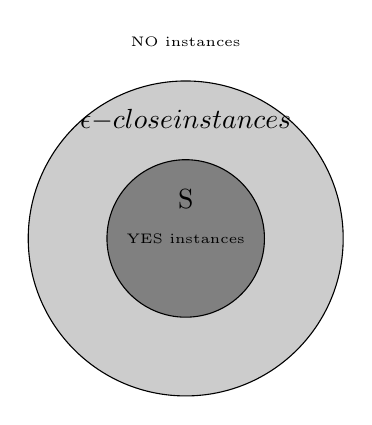
\begin{tikzpicture}
 
% Set A
\node [draw,
    circle,
    minimum size =4cm,
    fill=black!20,
    ] (A) at (0,0){};
 
% Set B
\node [draw,
    circle,
    minimum size =2cm,
    fill=black!50,
    ] (B) at (0,0){\tiny{YES instances}};

\node (C) at (0,2.5) {\tiny{NO instances}};
\node (D) at (0,1.5) {\(\tiny{\epsilon \text{-close instances}}\)};
\node (D) at (0,0.5) {S};
 
\end{tikzpicture}
}
\caption{Taxonomy of different instance types}
\end{figure}

To conclude, figure \ref{fig:taxonomy} gives a visual explanation to the property testing problem, in middle in have a dark-grey circle denoting the property \(S\) it self. 
In the light grey area surrounding it we have those instances which are \(\epsilon\)-close the being in \(S\). 
These are the instances for which our tester gives no guarantee about its output. 
Outside of the light grey area we have the \(\epsilon\)-far instances for which the tester will output a NO with high probability.

%
%
%

\section{Majority Porperty}

The majority property is the set of all binary vectors such that strictly more than half of the entries are 1. 
More formally, the \emph{weight} of a vector \(x\) is defined as \(\text{wt}(x) = \sum_{i=1}^{\abs{x}}x_i\) and the majority property is the following set, \[MAJ = \cbraces{x | \text{wt}(x) > \frac{\abs{x}}{2}}\]

\begin{proposition}
    There exists a \(O\braces{\frac{1}{\epsilon^2}}\)-time algorithm that distinguishes between \(x\in\) MAJ and \(x\) that is \(\epsilon\)-far from MAJ.
\end{proposition}

\begin{proof}
    We will use Chernoff's Bound (from theorem \ref{thm:chernoff_bound}).
    Our algorithm will query \(O\braces{\frac{1}{\epsilon^2}}\) random locations and acceptt iff  the fraction of sampled 1s (denoted \(\tilde{p}\)) is at least \(\frac{1-\epsilon}{2}\).

    Denote by \(p\) the actual fraction of 1s in the given instance \(x\).
    According to Chernoff's Bound, with probability \(\geq 2/3\) the following inequality holds: \(\abs{\tilde{p}-p} \leq \epsilon/2\).
    According to the definition of majority, if \(x \in \text{MAJ}\) then \(p > 1/2\).

    Since \(\abs{\tilde{p}-p}<\epsilon/2\) with probability 2/3, we get that \(\tilde{p} > \frac{1-\epsilon}{2}\) with probability \(\geq 2/3\).

    If \(x\) is \(\epsilon\)-far from MAJ, \(p<1/2-\epsilon\), so we get that \(\tilde{p} < \frac{1-\epsilon}{2}\) with probability \(\geq 2/3\).
    
    Therefore, if we accept only when \(\tilde{p}\) is more than \(\frac{1-\epsilon}{2}\) we are correct with probability \(\geq 2/3\).
\end{proof}

Before moving on we emphasize an important part in the definition of a tester. 
Recall that a tester much succeed in probability of at least \(2/3\) for \textbf{each} instance \(x\).
In other words, for each \(x\) at least \(2/3\) of the coin tossess the tester makes will result a YES output if \(x\) has the property and at least \(2/3\) of the coin tossess wil result a NO output if \(x\) is at least \(\epsilon\) far from having the property.

\begin{proposition}
    Any randomized algorithm that exactly decides MAJ (even for \(\epsilon\)-close instances) must do \(\Omega(n)\) queries.
\end{proposition}

\begin{proof}
    Let \(D_1\) be a distribution over instances that do not possess the property (including the \(\epsilon\) close instances) which is uniform over the strings with hamming weight of \emph{exactly} \floor{n/2}.
    Let \(D_2\) be a distribution of the instances that  possess the property which is uniform over the strings with hamming weight of \emph{exactly} \(\floor{n/2} + 1\).

    Let's assume the following lemma holds, later we will prove it as well.
    \begin{lemma}\label{lemma:second_proposition_lemma}
    Any randomized algorithm \(A\) that makes \(q\) queries to the input and for the random variables \(X_n\) sampled from \(D_1\) and \(Y_n\) sampled from \(D_2\) the following holds:
    \[
    \abs{\pr{A\braces{X_n} = 1} - \pr{A\braces{Y_n} = 1}} \leq \frac{q}{n}
    \]
    \end{lemma}

    Assuming Lemma \ref{lemma:second_proposition_lemma} holds, if \(q \ll n\), the probability of successfully distinguishing between \(X_n\) and \(Y_n\) is small.
    In particular, for any algorithm \(A\) that makes less than \(n/3\) quries, it holds that:
    \[
        \abs{\pr{A\braces{X_n} = 1} - \pr{A\braces{Y_n} = 1}} < \frac{1}{3}
    \]
    Therefore either \(\pr{A\braces{X_n} = 1} > 1/3\) or \(\pr{A\brackets{Y_n} = 1} < 2/3\)
    Notice that the probabilities above are taken over all coin tosses of \(A\) and over the sampling of \(X_n\) and \(Y_n\). Thus, from averaging arguments, at least one of the following must hold:
    \begin{itemize}
        \item There is an \(x\) with weight \floor{n/2} such that \(\pr{A\of{x} = 1} > 1/3\)
        \item There is an \(x\) with weight \(\floor{n/2} + 1\) such that \(\pr{A\of{x} = 1} < 2/3\).
    \end{itemize} 

\end{proof}

Now let's prove Lemma \ref{lemma:second_proposition_lemma}.
\begin{proof}
    Assume that there is some algorithm \(A\) for which the Lemma doesn't hold.
    To prove the lemma, we have to show that when the algorithm is fed with instances distributed from \(D_1\) and when it is fed with instances from \(D_2\) the algorithm can't distinguish between the two distributions with probability greater than \(q/n\).
    Let $X_n$
\end{proof}

\begin{proposition}
    Any deterministic algorithm that distinguishes between instances in MAJ and instances that are 0.5-far from MAJ, must make at least \(\frac{n}{2}\) queries.
\end{proposition}

\begin{proof}
    Assume there exists such algorithm \(A\) that makes \(q < n/2\) queries.
    Consider the execution of \(A\) such that each query is answered with 0. 
    This execution is consistent with the all "0" string.
    It is also consistent with a string whose hamming weight is \(n-q\) ("1" on any position not queried).
    Since \(q<n/2\), this vectors hamming weight is \(>n/2\) and thus the algorithm will be wrong on this input.
\end{proof}

\section{Testing Symmetric Properties}

We first define what a symmetric property is.
\begin{definition}
    A property on binary sequence is symmetric if it for each \(x,y\) with the same hamming weight either both \(x,y \in S\) or \(x,y \not \in S\).
\end{definition}

\begin{theorem}
    For any symmetric property of binary sequences \(S\) there exists a randomized algorithm that makes \(O\of{1/\epsilon^2}\) queries and distringuishes between \(x \ in S\) and \(x\) that is \(\epsilon\)-far from \(S\).
\end{theorem}

Notice, therefore, that one can decide if \(x \in S\) or not by known the hamming weight of \(x\).
More formally: 
\[
    \forall n \exists W_n \subseteq \brackets{n} s.t \forall x \in \cbraces{0,1}^n, x\in S \iff \text{wt}(n) \in W_n
\]


\begin{algorithm}[t]\label{alg:symmetric_tester}

\Begin{
    Let \(n \leftarrow \abs{x}\)
    Query \(x\) at \(m=\Theta\of{1/\epsilon^2}\) locations. \\
    Let \(\tilde{p}\) be the fraction of sampled location equal to 1. \\ 
    Accept iff \(\exists w \in W_n\) such that \abs{\tilde{p} - \frac{w}{n}}
}
\caption{Symmetric Property Tester}
\end{algorithm}

The tester is given at algorithm \ref{alg:symmetric_tester}.
The correctness of the algorithm follows from the proof for the MAJ property and from Chernoff Bound.